\documentclass{EESD}
% To change the slides size go to EESD.cls file and edit the preamble as explained.

% ---- Add your Meta-data to the PDF (Copyrights Kinda!) ----
\hypersetup{
  pdfinfo={
    Title={Light Rail and Park\&Ride facilities in Sioux Falls},
    Author={Julien Ars},
  }
}

% Important packages to be called
\usepackage{subcaption} % for adding sub-figures
\usepackage{graphicx}
\usepackage{tikz} % for cool graphics and drawings

\usepackage[absolute,overlay]{textpos} % To place the figures by coordinates (x,y) - Beamer doesn't support floats XD
\usepackage{multicol} % To adjust items and stuff automatically in a number of a pre-specified columns
\graphicspath{{Figures/}}
\usepackage[utf8]{inputenc}
\usepackage{amsmath}
\usepackage{amsfonts}
\usepackage{amssymb}
\usepackage{lipsum} % Just a dummy text generator
\usepackage{hyperref}
% fonts packages
\usepackage{ragged2e} % Justified typesetting

% ChatGPT for table
\usepackage{booktabs}
\usepackage{multirow}
\usepackage{adjustbox}
\usepackage{pifont}
\usepackage{array}

\usepackage{algorithm}
\usepackage{algpseudocode}
\usepackage{xcolor}

% For References Only
% \usepackage[style=authortitle,backend=bibtex]{biblatex}
% \addbibresource{references.bib} % Call the references database
% \AtBeginBibliography{\tiny} % Specify font size (Size matters)
\renewcommand{\footnotesize}{\tiny}

% For adding code blocks
\usepackage{listings}
\lstset
{
    language=[LaTeX]TeX,
    breaklines=true,
    basicstyle=\tt\scriptsize,
    keywordstyle=\color{blue},
    identifierstyle=\color{magenta},
    commentstyle=\color{red},
    rulecolor=\color{black},
    numbers=left,
    numberstyle=\tiny\color{black},
    % framexleftmargin=15pt,
    frame = single,
}

\author{Julien Ars}
\title[Light rail and P\&R facilities in Sioux Falls]{Light Rail and Park\&Ride facilities in Sioux Falls}

\institute[ENAC]{{\'Ecole Polytechnique F\'ed\'erale de Lausanne (EPFL)}{\newline\newline Civil Engineering}}
\subject{Talk}
\date{2025-05-28}

\begin{document}

{ % <-- don't forget the scope resolution (Brackets) to limit the background change only for the cover page; otherwise, it will override the whole document's background :)
\usebackgroundtemplate{} % To add a background for this slide XD - Empty one
\coverpage{
\titlepage{~}
% To add additional text to the title components 
{\newline \small CIVIL-477 - Transport Networks Modelling \& Analysis}
}
} % <-- and yeah close them too :)


\setbeamertemplate{logo}{} % To override the logo from the other slides and delete it completely

% Use smart division for the TOC
\section*{Table  of content}
\begin{frame}{Outlines}
\tableofcontents
\end{frame}

% -----------------------				Introduction
\section{Introduction}
\breakingframe{
\begin{textblock*}{0.8\textwidth}[0,0.5](0.17\textwidth,  0.55\textheight)
\centering \Huge\textbf{\textcolor{black}{Introduction}}
\end{textblock*}
}

\subsection{Sioux Falls}
\begin{frame}{Sioux Falls}
	\begin{columns}
	\column{0.5\textwidth}
	\begin{itemize}
		\item Most populous city in South Dakota
		\item<2-> More than 200'000 inhabitants (rapidly growing : 125 000 in 2000) \footnote{Source : Wikipedia}
		\item<3-> Superficy of 210 km$^2$
		\item<4-> Nice waterfalls
		\item<5-> 9 bus lines ! Run 6 days per week, $\approx$ every 30 min.
		\item<5-> Public on-demand service to supplement the bus lines.
	\end{itemize}
	\column{0.5\textwidth}
	\includegraphics<1>[width = \linewidth]{sioux-falls-map.png}
	\includegraphics<2-3>[width = \linewidth]{SiouxFalls-GoogleEarth.PNG}
	\includegraphics<4>[width = \linewidth]{sioux_falls_falls_park.jpg}
	\includegraphics<5>[width = \linewidth]{siouxfalls_bus_network.png}
	\end{columns}

\end{frame}

\subsection{Adding a light rail}
\begin{frame}{Adding a light rail}
	\begin{columns}
	\column{0.5\textwidth}
	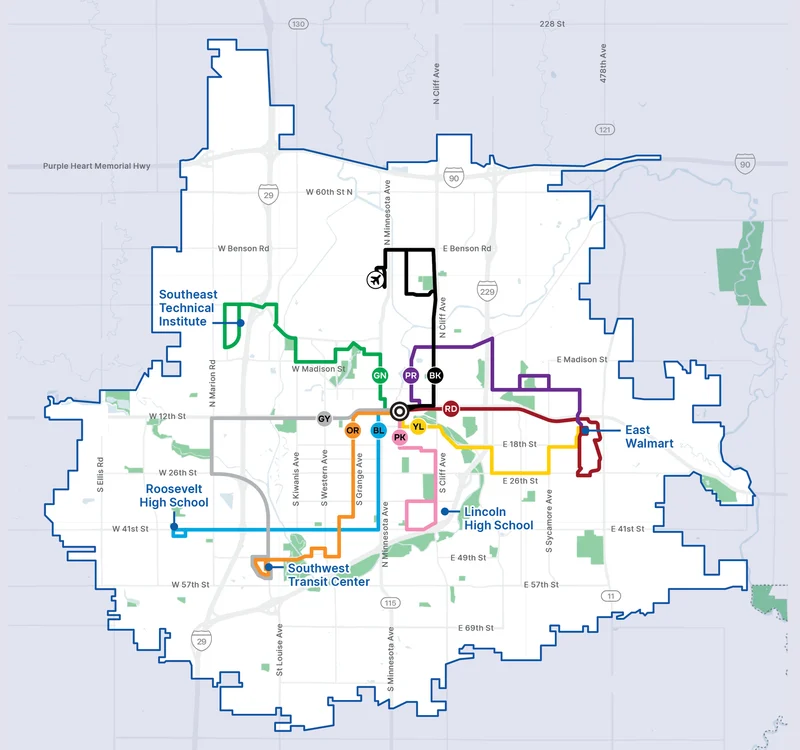
\includegraphics[width = \linewidth]{siouxfalls_bus_network.png}
	\column{0.5\textwidth}
	\begin{itemize}
		\item Now let's imagine the city of SiouxFalls decides to enter in the 21st century
		\item And want to replace a bus line by a light rail line with Park \& Ride facilities.
		\item What will be the impact on the trafic ?
	\end{itemize}
	\end{columns}
\end{frame}

\begin{frame}{Our study}
	Considering the classic 'Sioux Falls' benchmark network, and the current bus network of the city of Sioux Falls.
	\begin{itemize}
		\item[\textrightarrow] Add light rail transit lines to match current bus lines and the most used road links.
		\item[\textrightarrow] Test the trafic conditions in the 3 cases : \begin{description}
			\item[Base] No light rail
			\item[Light Rail] Light rail can only be taken when origin and destination is served by the network.
			\item[P\&R] Light rail can only be taken when origin \textbf{or} destination is served by the network.
		\end{description}
		\item[] 
	\end{itemize}
\end{frame}


% --------------------------------------------- Methodology

\section{Methodology}
\breakingframe{
\begin{textblock*}{0.8\textwidth}[0,0.5](0.17\textwidth,  0.55\textheight)
\centering \Huge\textbf{\textcolor{black}{Methodology}}
\end{textblock*}
}

\subsection{Defining transit lines}
\begin{frame}{Defining transit lines}
	\begin{columns}
		\column{0.5\textwidth}
		\centering
		\begin{enumerate}
			\item<1-2> Match the classic SiouxFalls network to the bus map \onslide<2>{(and vice-versa)}
			\item<3> Compare with the \alert{Base} situation to identify the most used road links.
			\item<4> Define transit lines
			\item<5> Compute distance and time of travel for the transit line
		\end{enumerate}
		\column{0.5\textwidth}
		\centering
		\begin{figure}
			\centering
			\only<1>{
			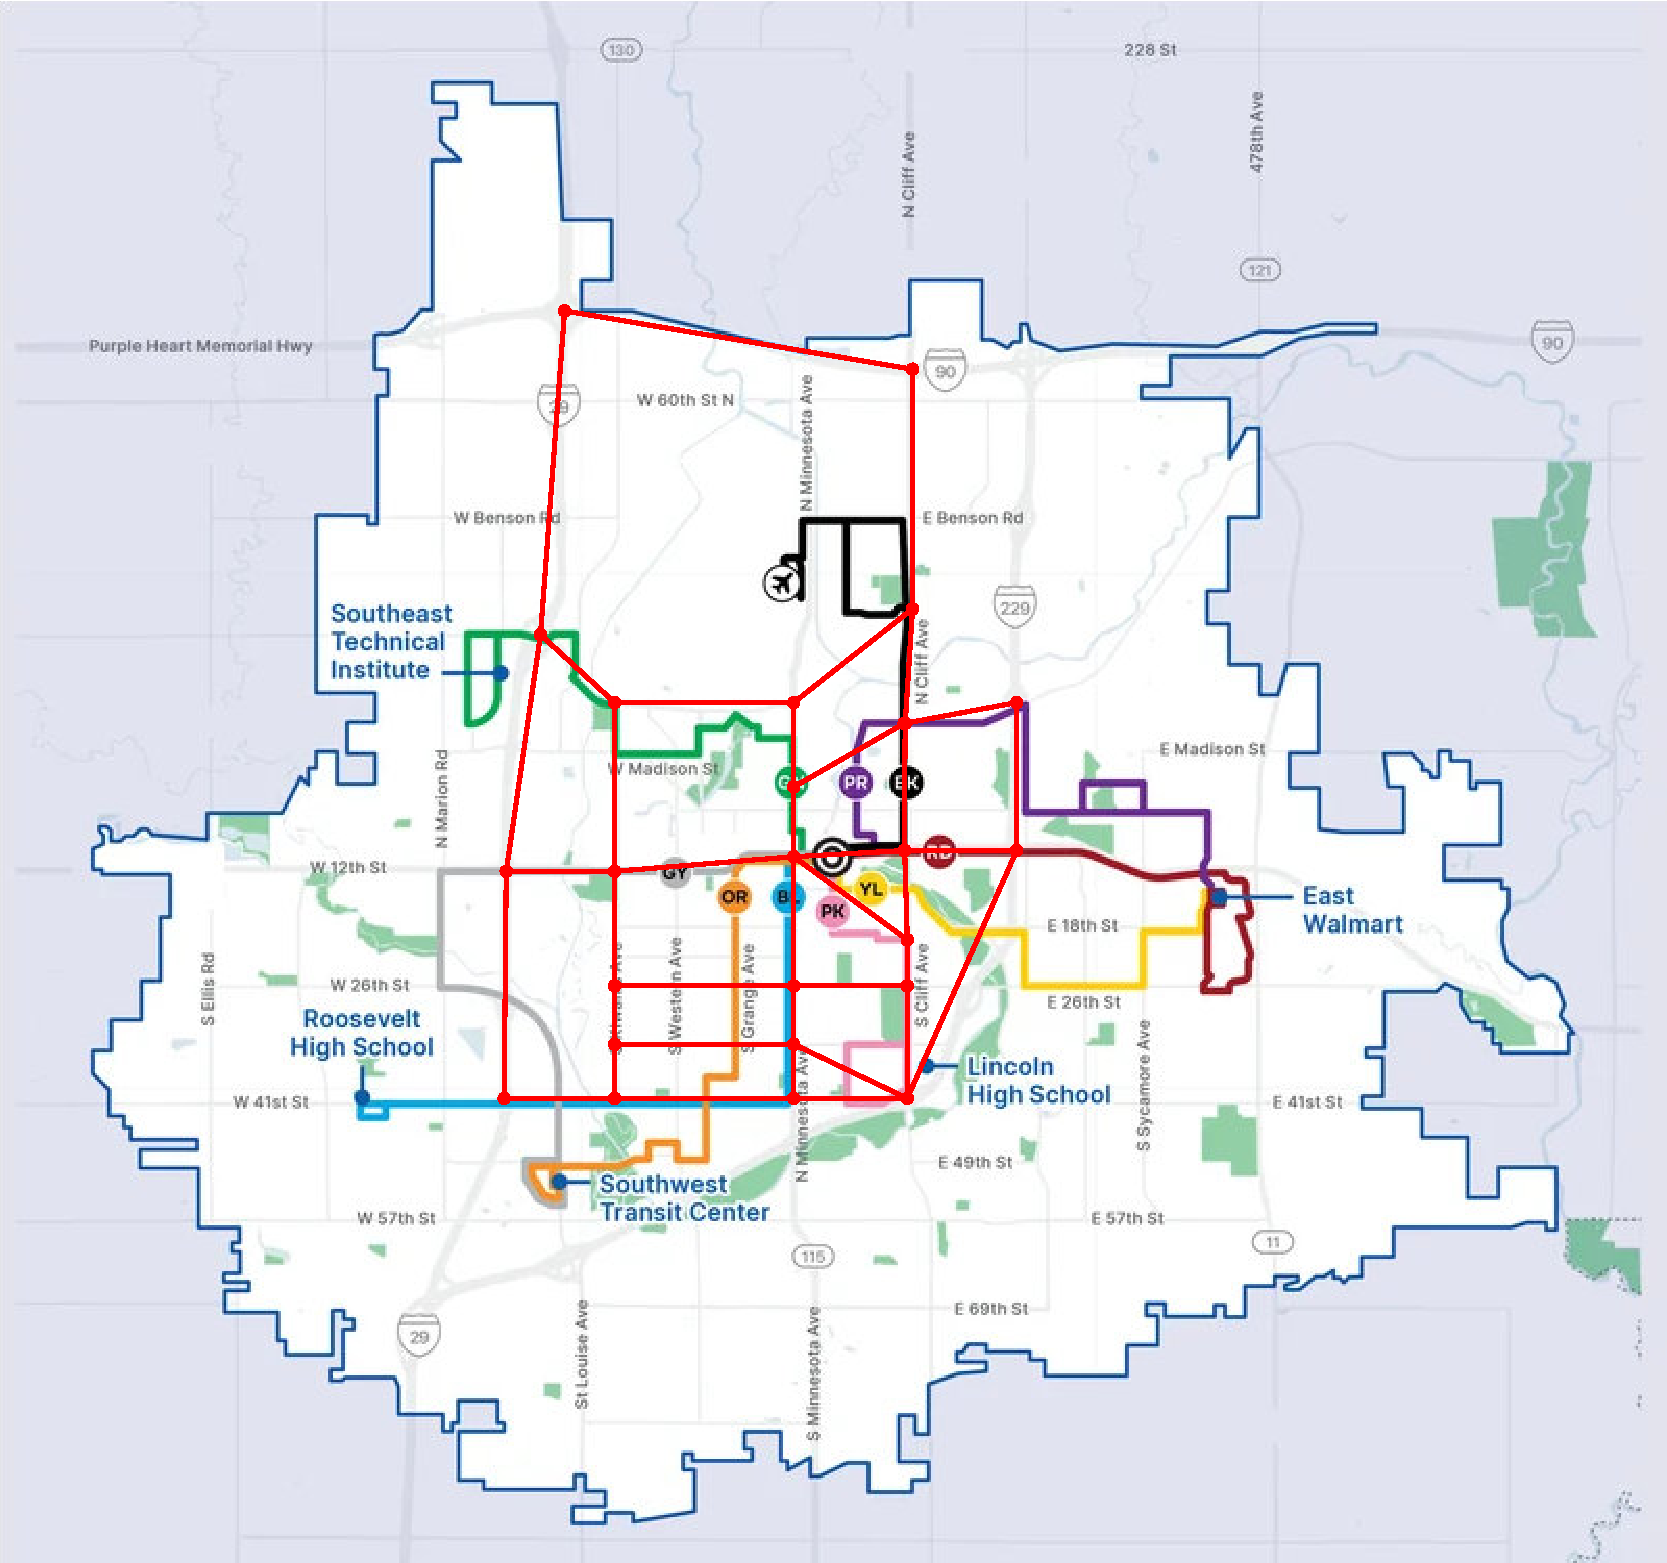
\includegraphics[width=0.75\textwidth]{road_network_on_bus_map.pdf}
			\caption{Sioux Falls nodes and edges matched on the bus map}
			}
			\only<2>{
			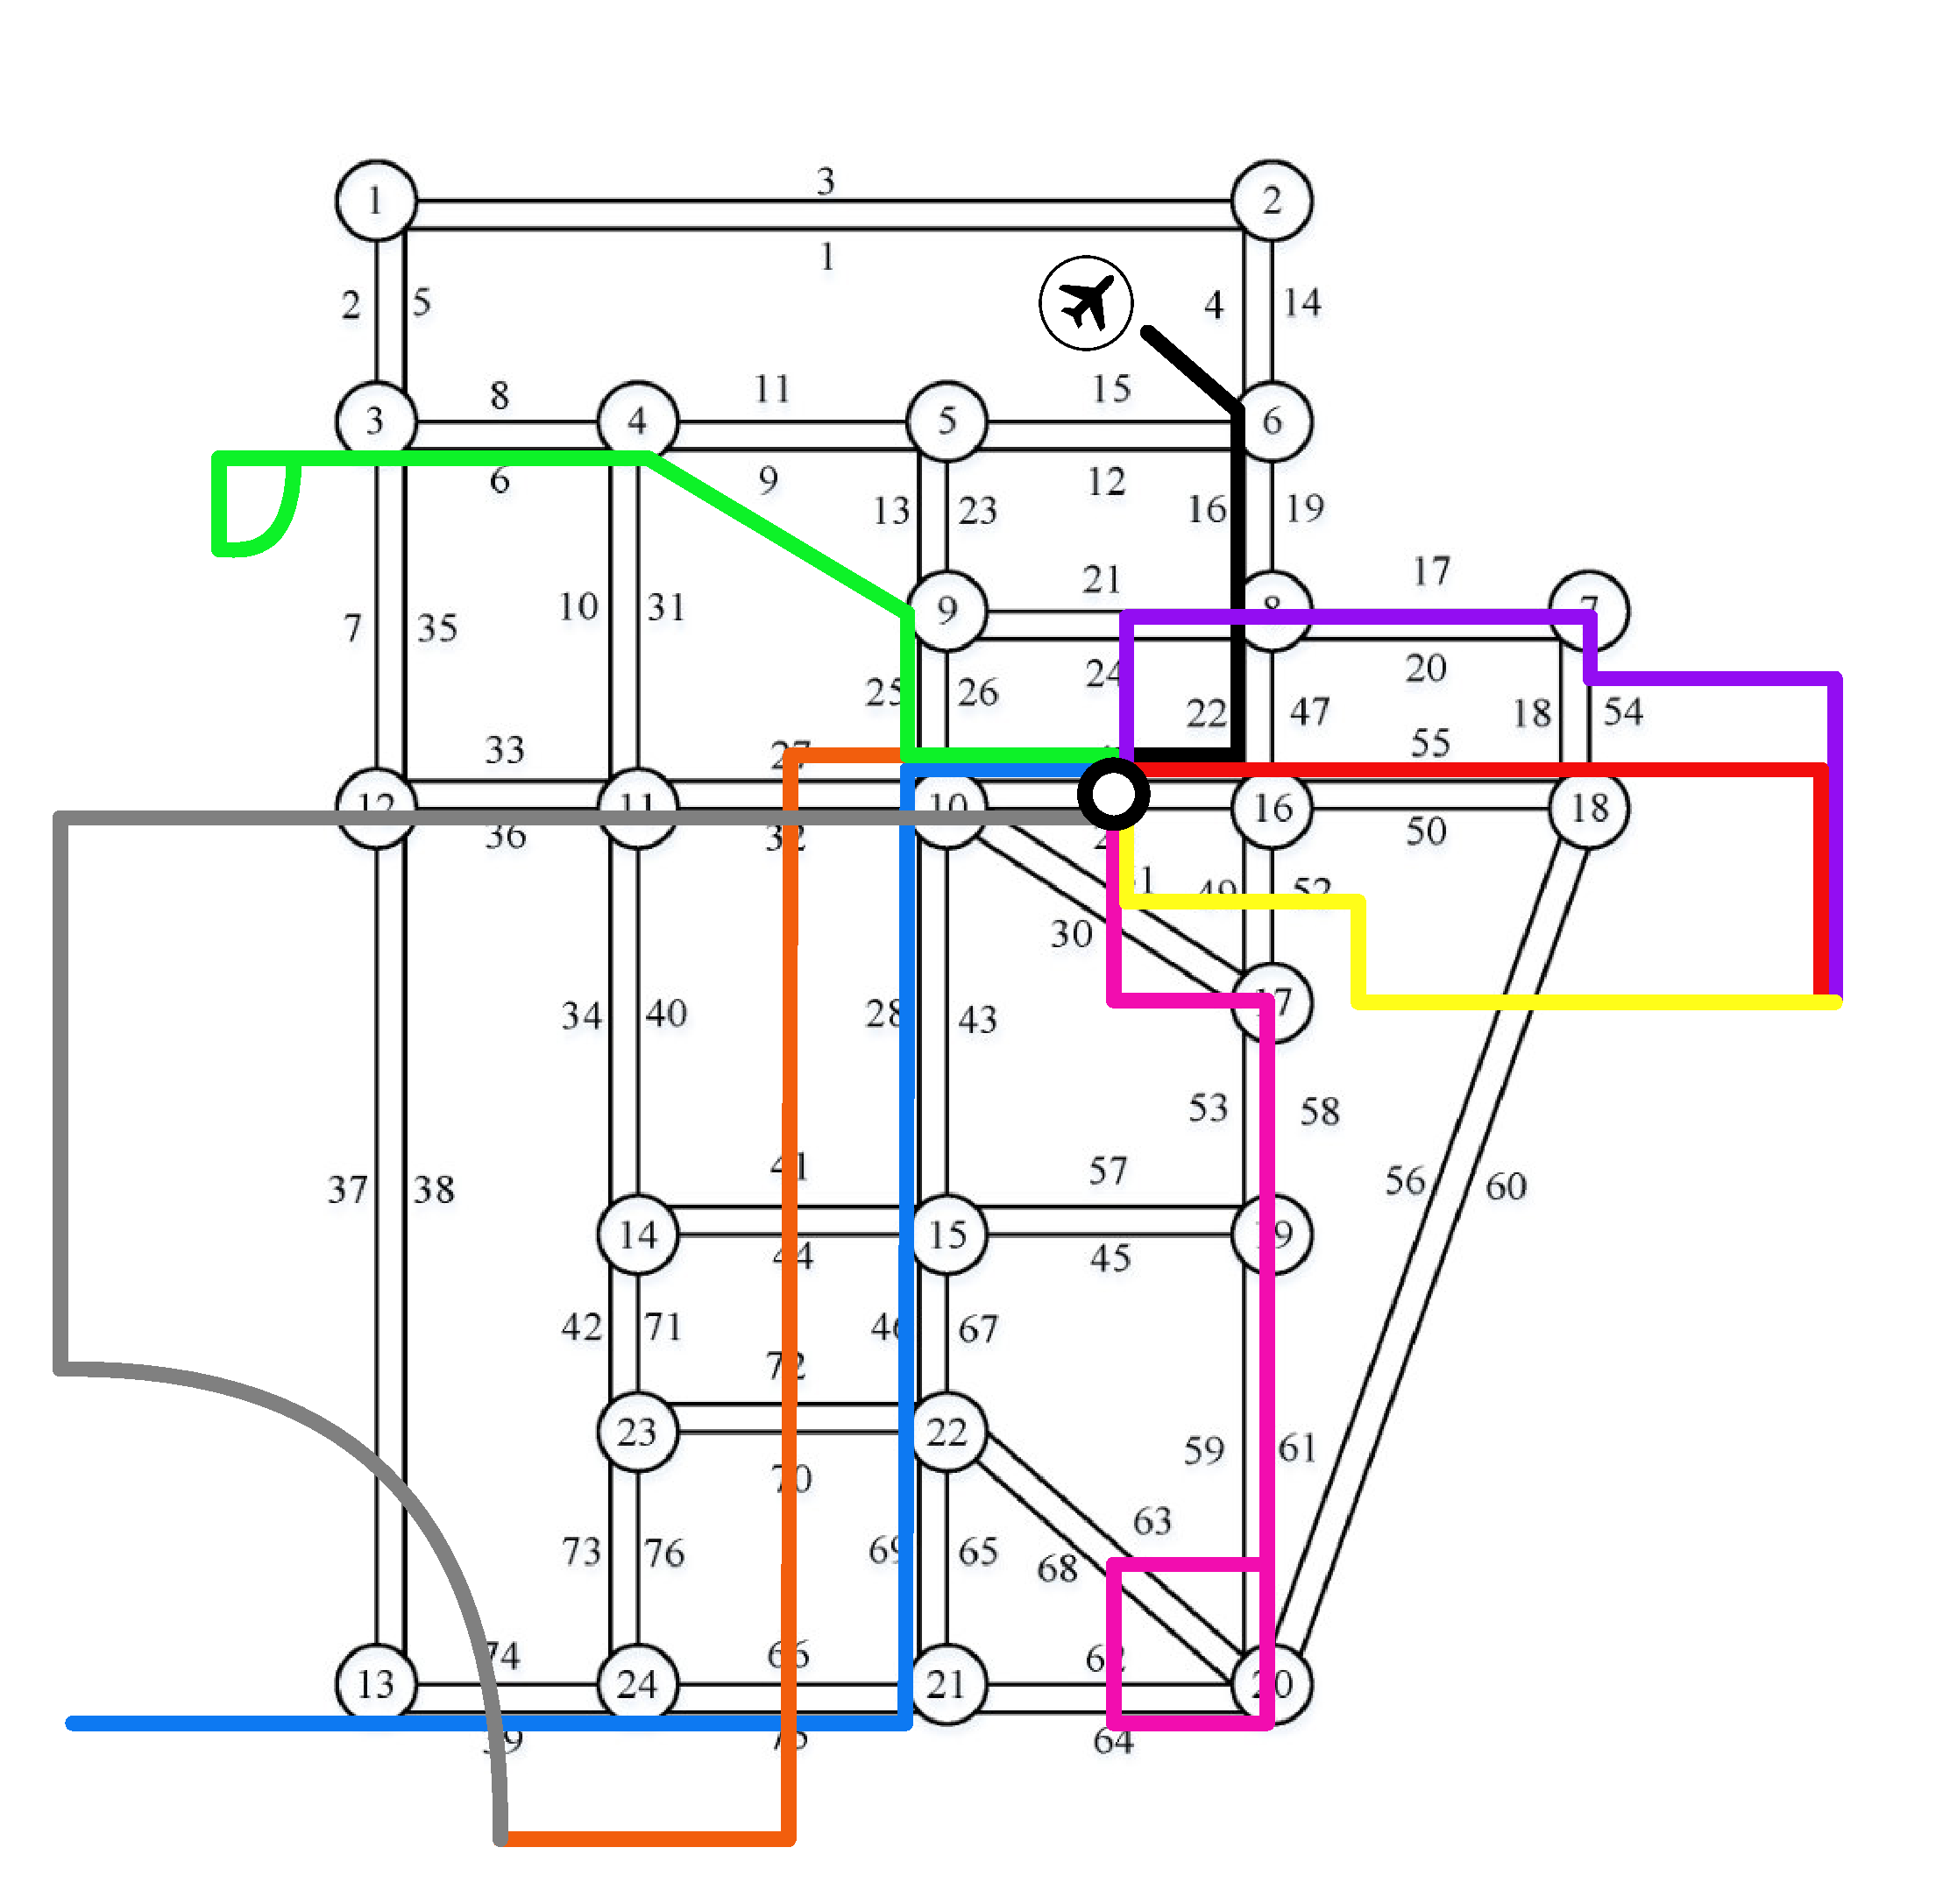
\includegraphics[width=0.75\textwidth]{bus_network_on_road_map.pdf}
			\caption{Sioux Falls bus lines matched on the classic network}
			}
			\only<3>{
			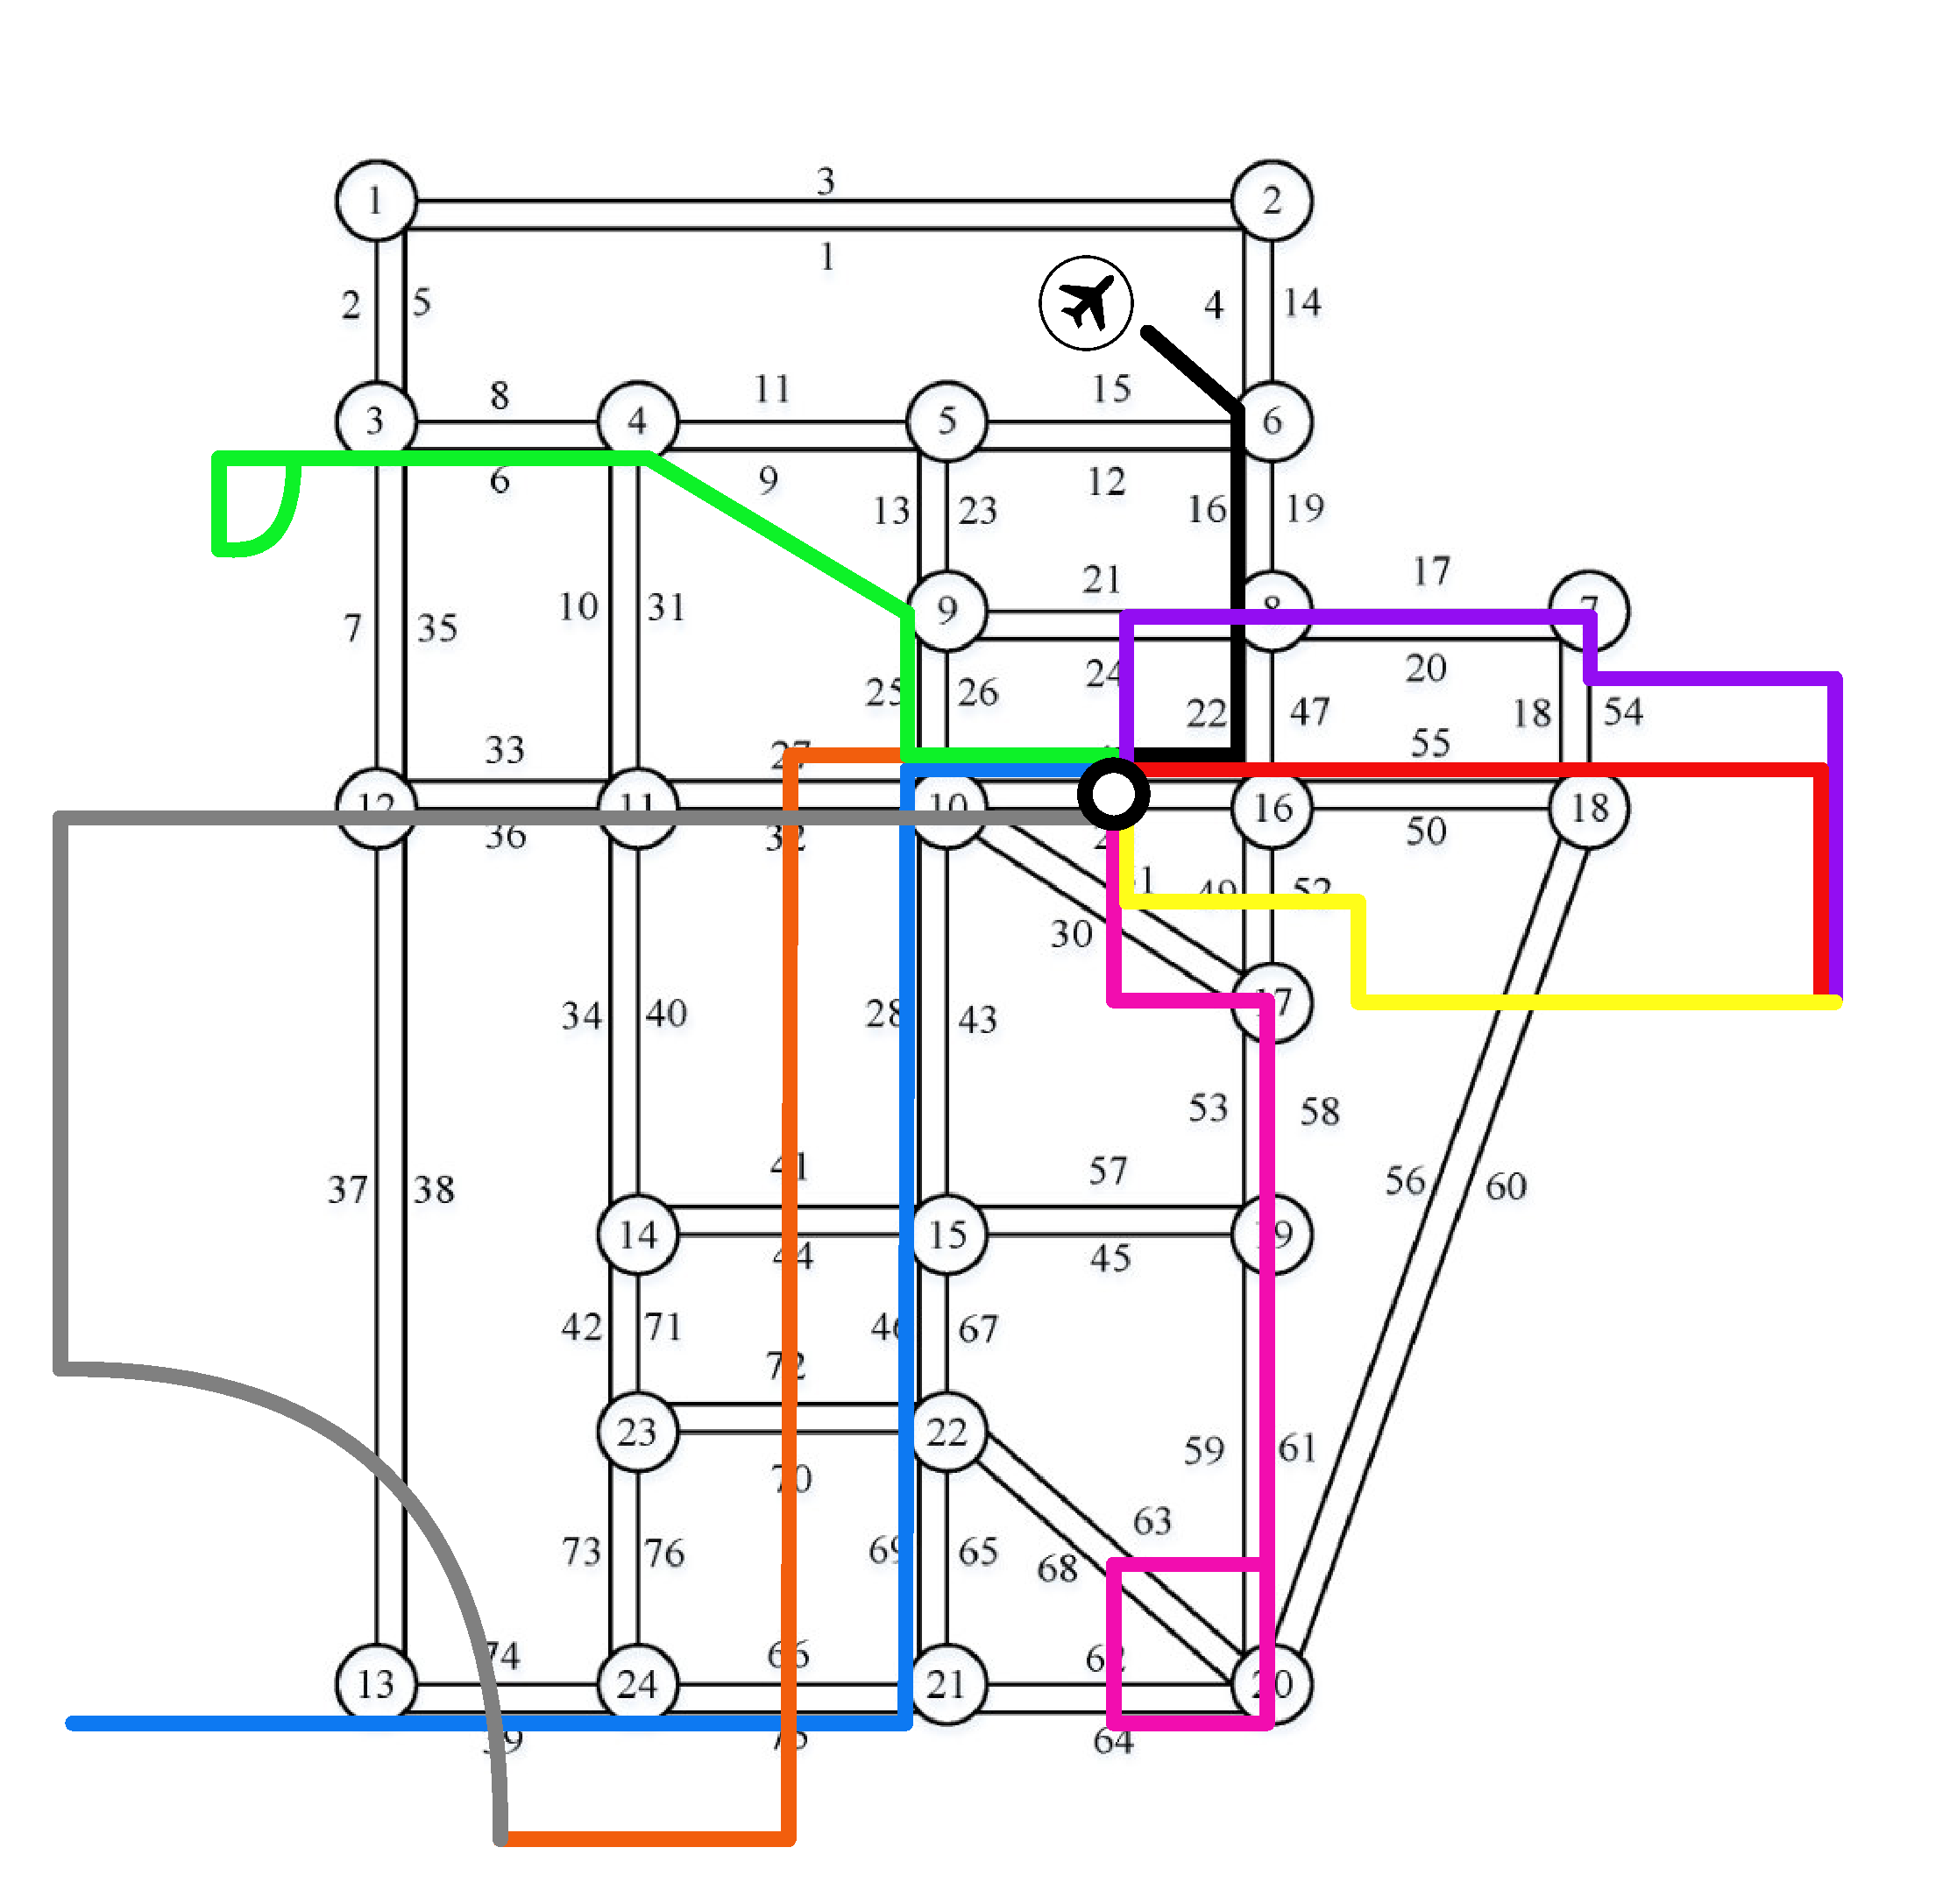
\includegraphics[width=0.75\textwidth]{bus_network_on_road_map.pdf}
			\caption{\alert{Base} trafic flows (at UE)}
			}
			\only<4-5>{
			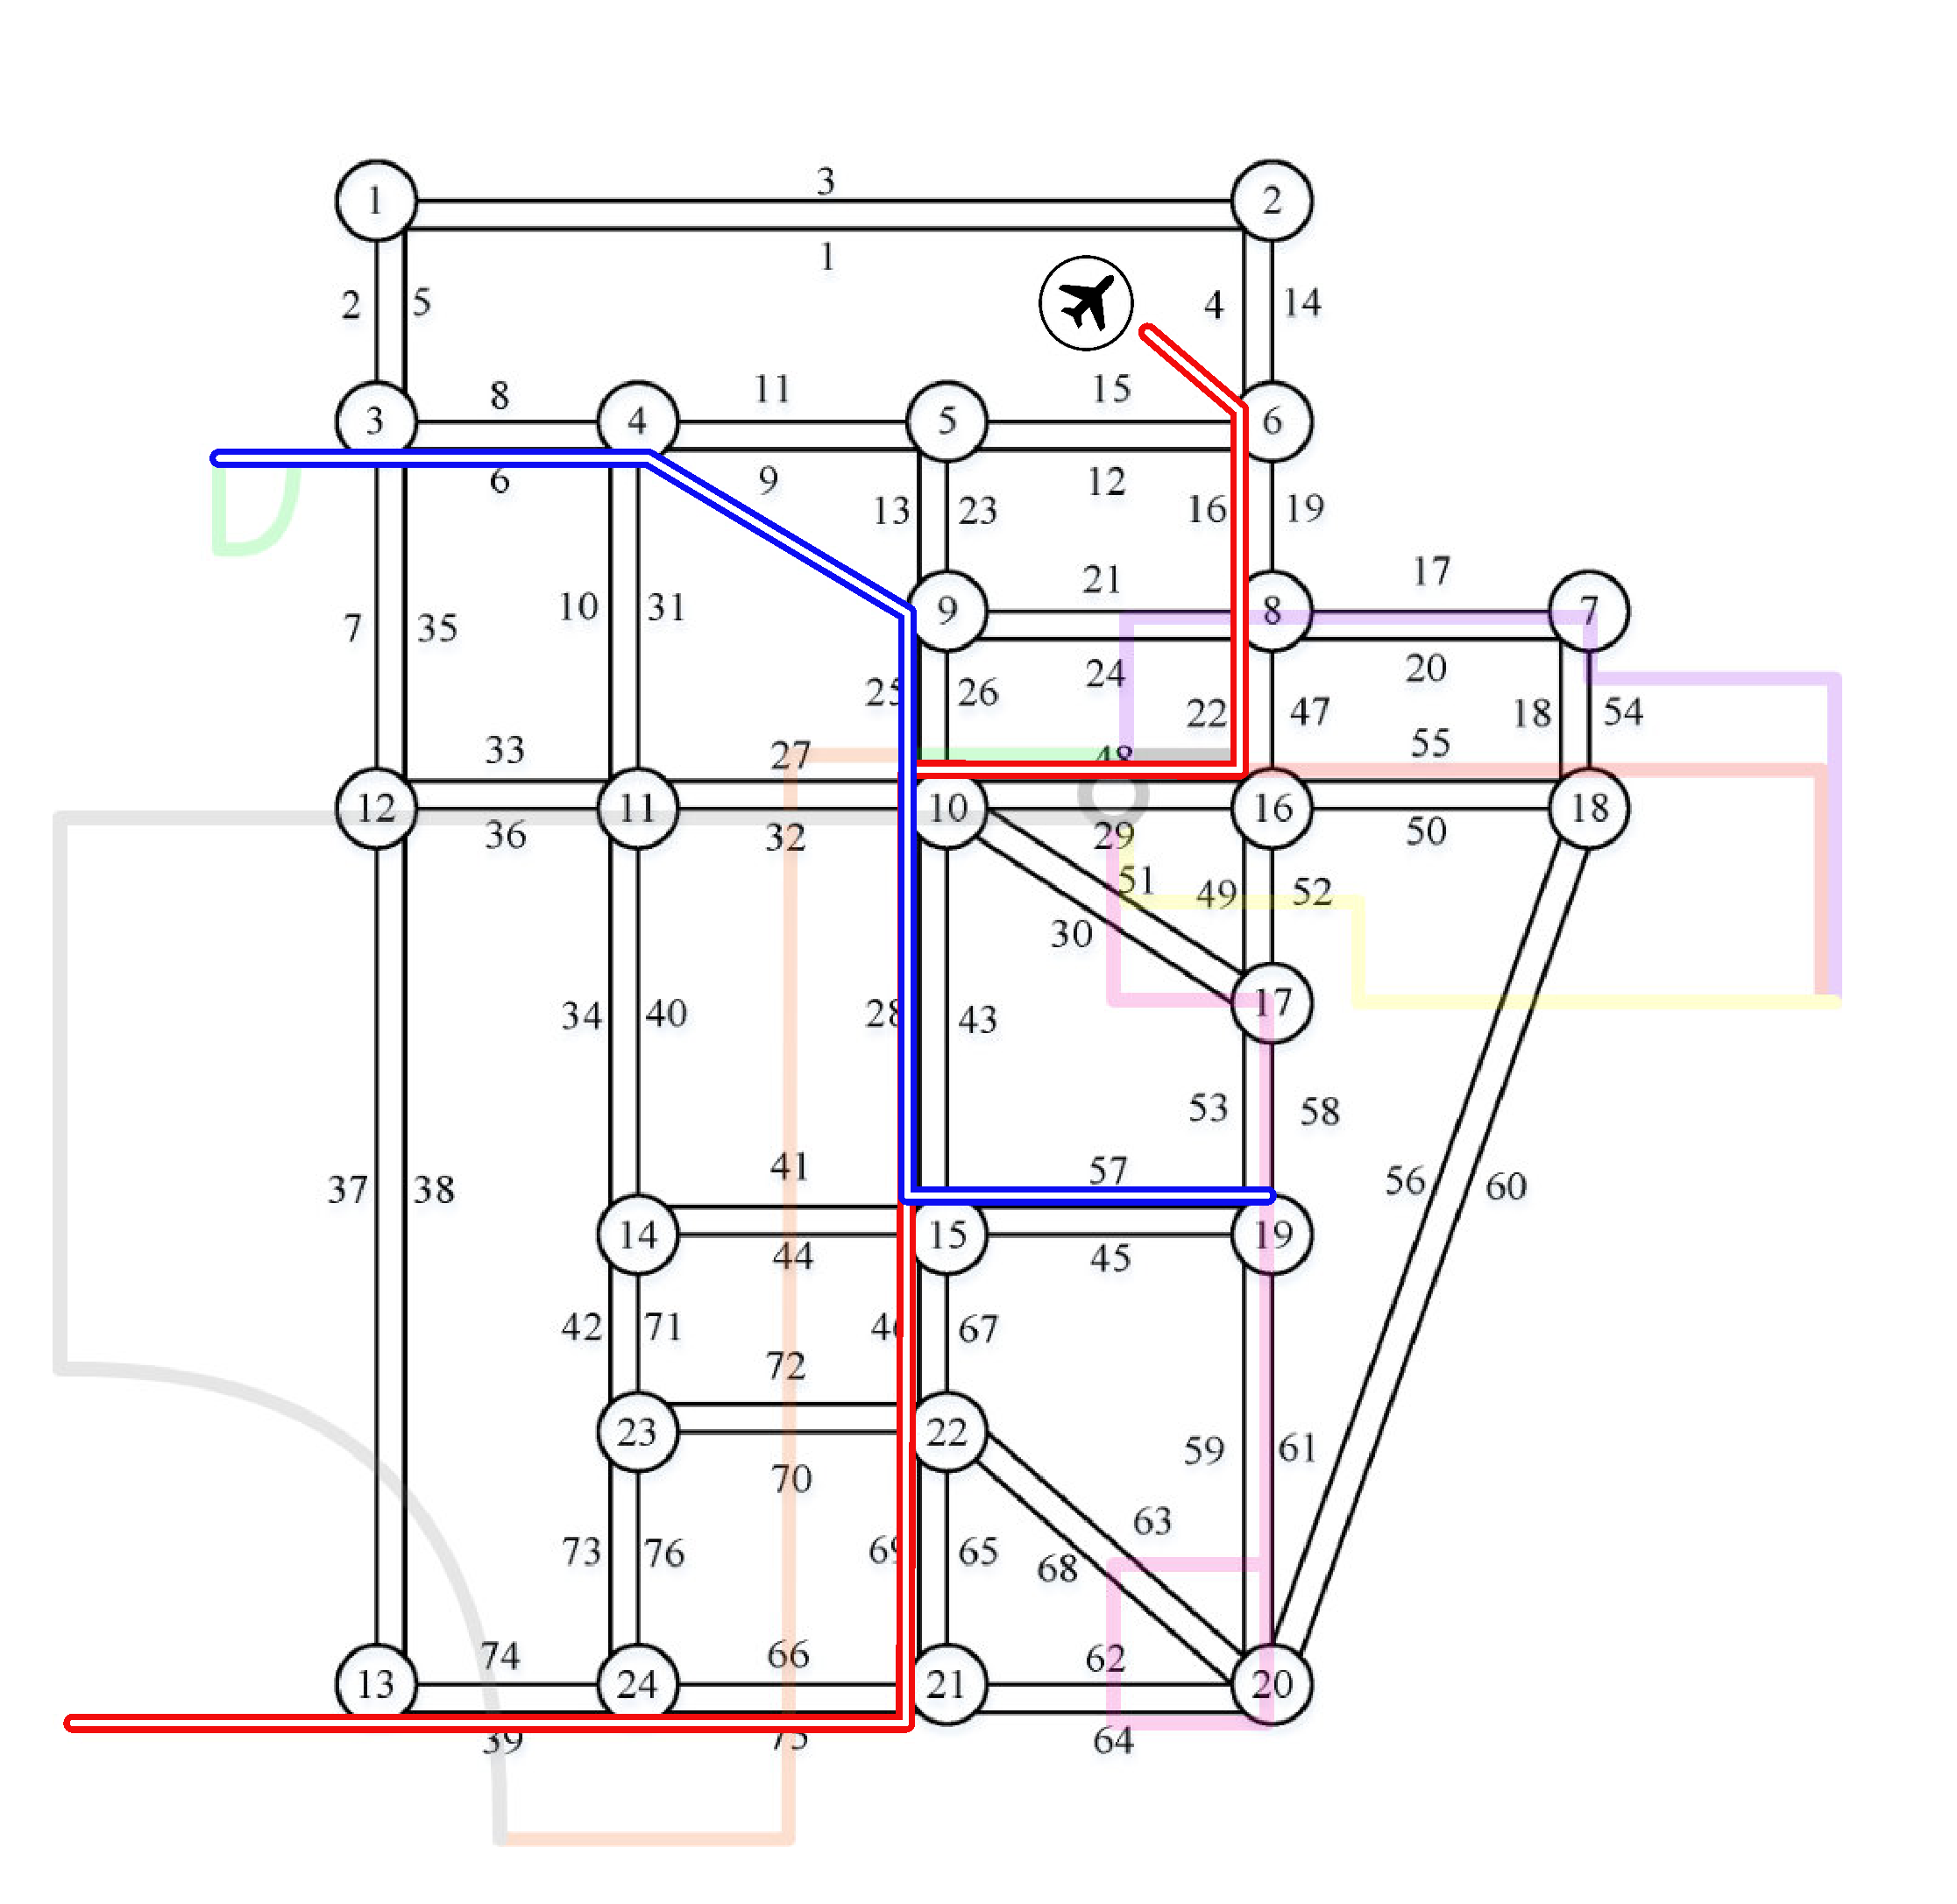
\includegraphics[width=0.75\textwidth]{two_lines.pdf}
			\caption{The two lines defined}
			}
		\end{figure}
	\end{columns}
\end{frame}

\subsection{Modelling trafic}
\begin{frame}{Modelling trafic (Base case)}
	Classic Frank-Wolf algorithm
	\begin{enumerate}
		\item Update travel times
		\item Descent direction (All-or-nothing assignment on the shortest path)
		\item Determine step (line search)
		\item Update link flows
	\end{enumerate}
\end{frame}

\begin{frame}{Modelling trafic (Light Rail case)}
	\begin{columns}
		\column{0.6\textwidth}
		Two layered approach
		\begin{itemize}
			\item The light rail network is another network
			\item For now : no connections between the two layers (no Park and Ride)
			\item<2> For groups where origin and destination on the light rail network: change all-or-nothing assignment. \begin{itemize}
				\item Compute the shortest path on both Networks
				\item Assign the trafic only on the one with the shortest time (can use the labels of Dijkstra)
			\end{itemize}
		\end{itemize}
		\column{0.4\textwidth}
		\centering
		\begin{figure}
			\centering
			\only<1>{
			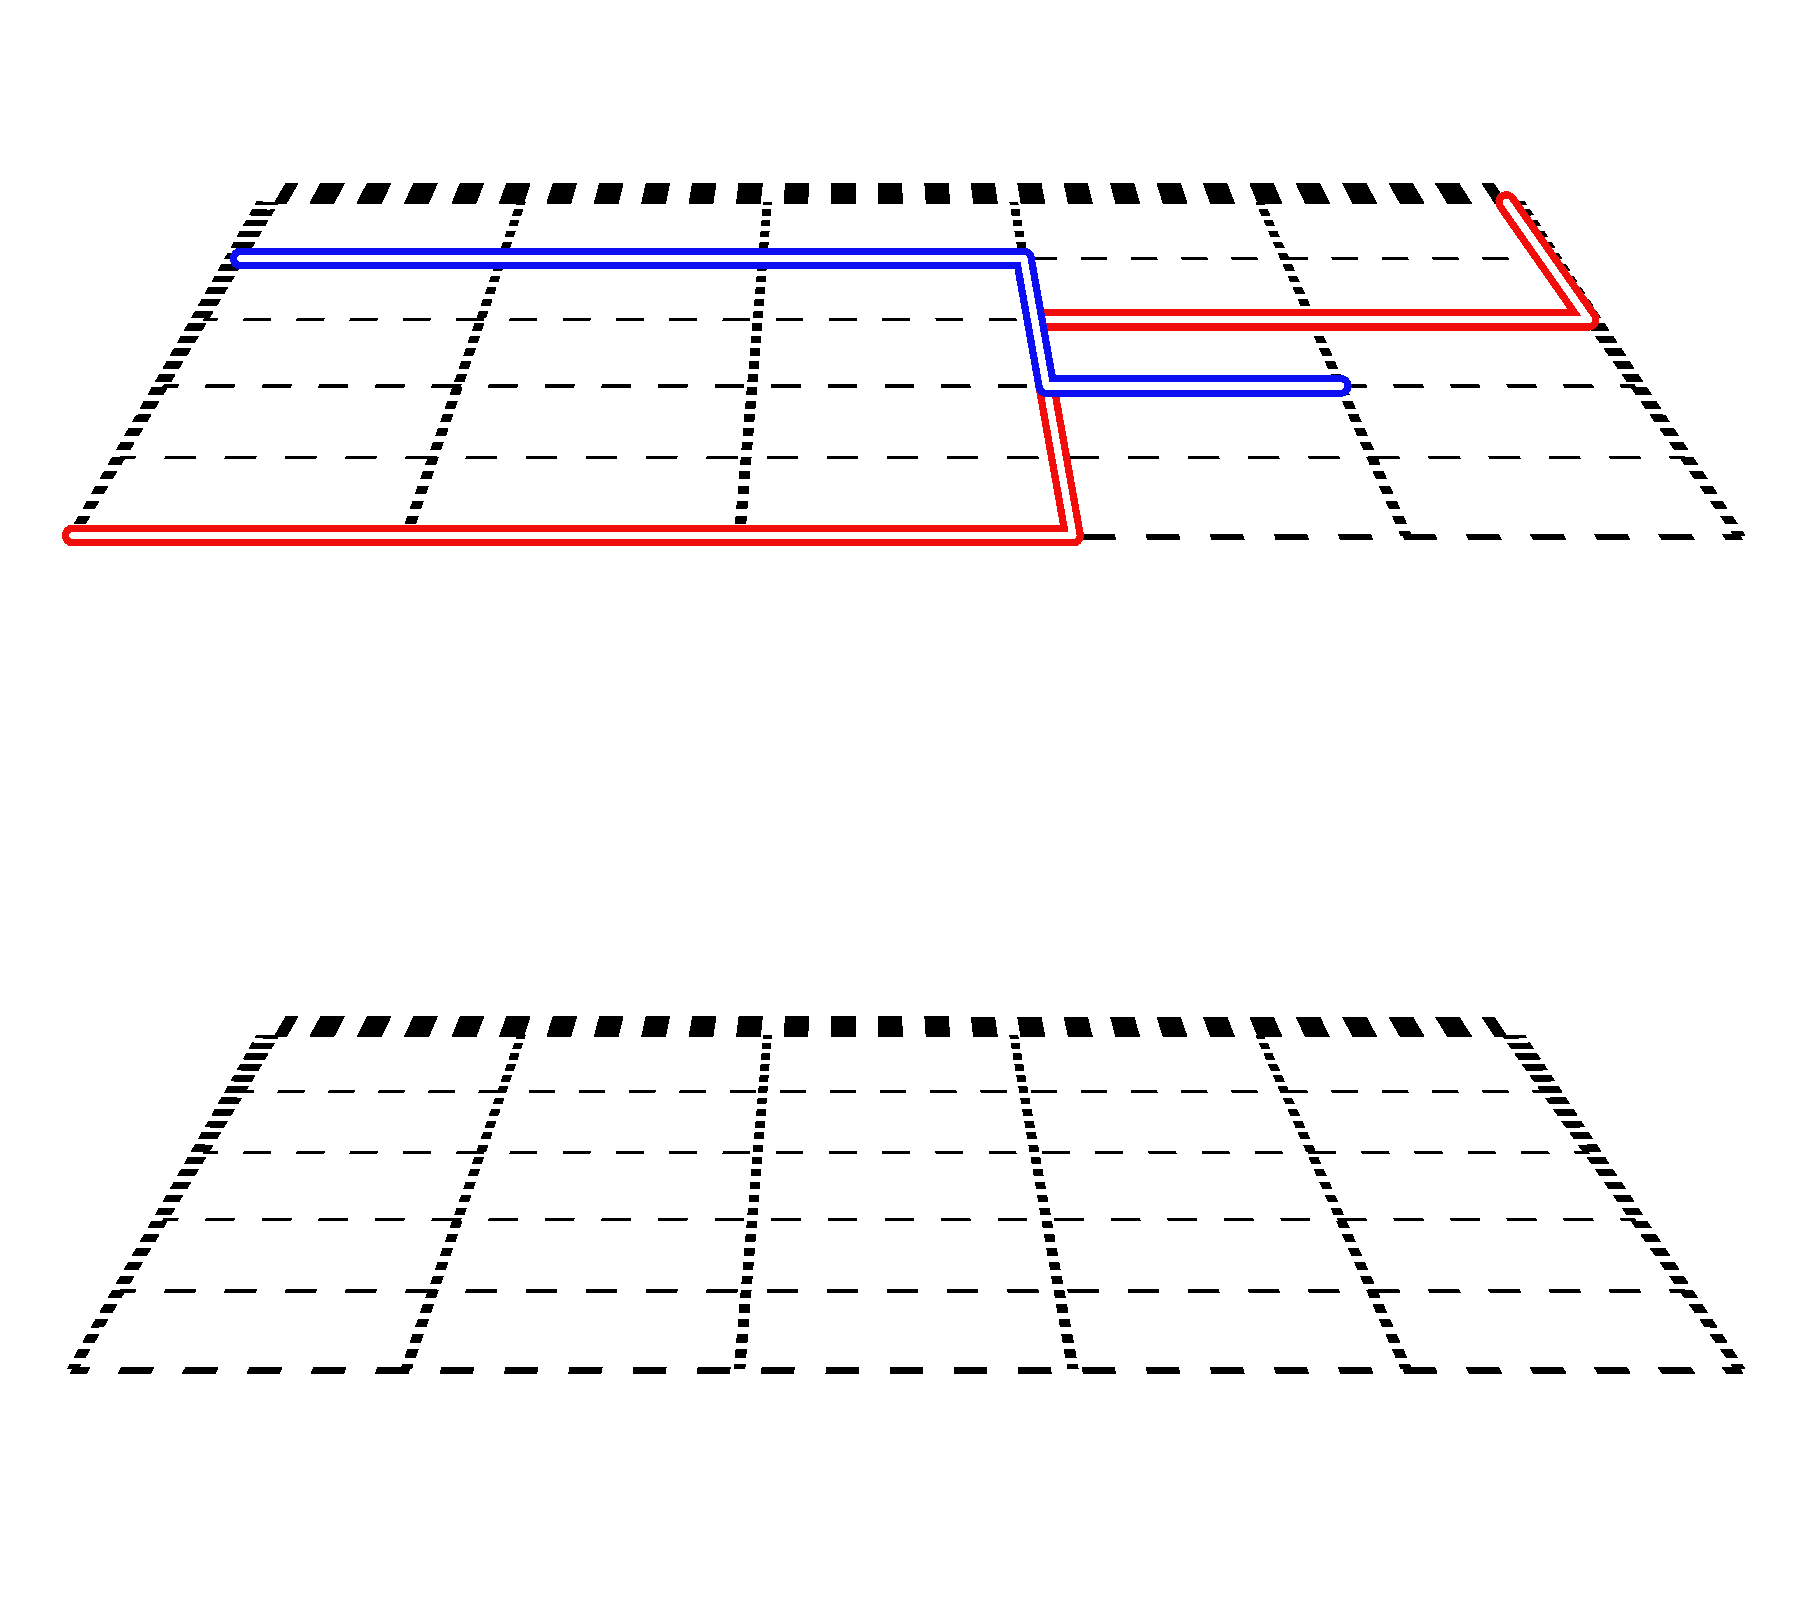
\includegraphics[width=\textwidth]{deux_layers_0.pdf}
			\caption{Two layers approach}
			} \only<2>{
			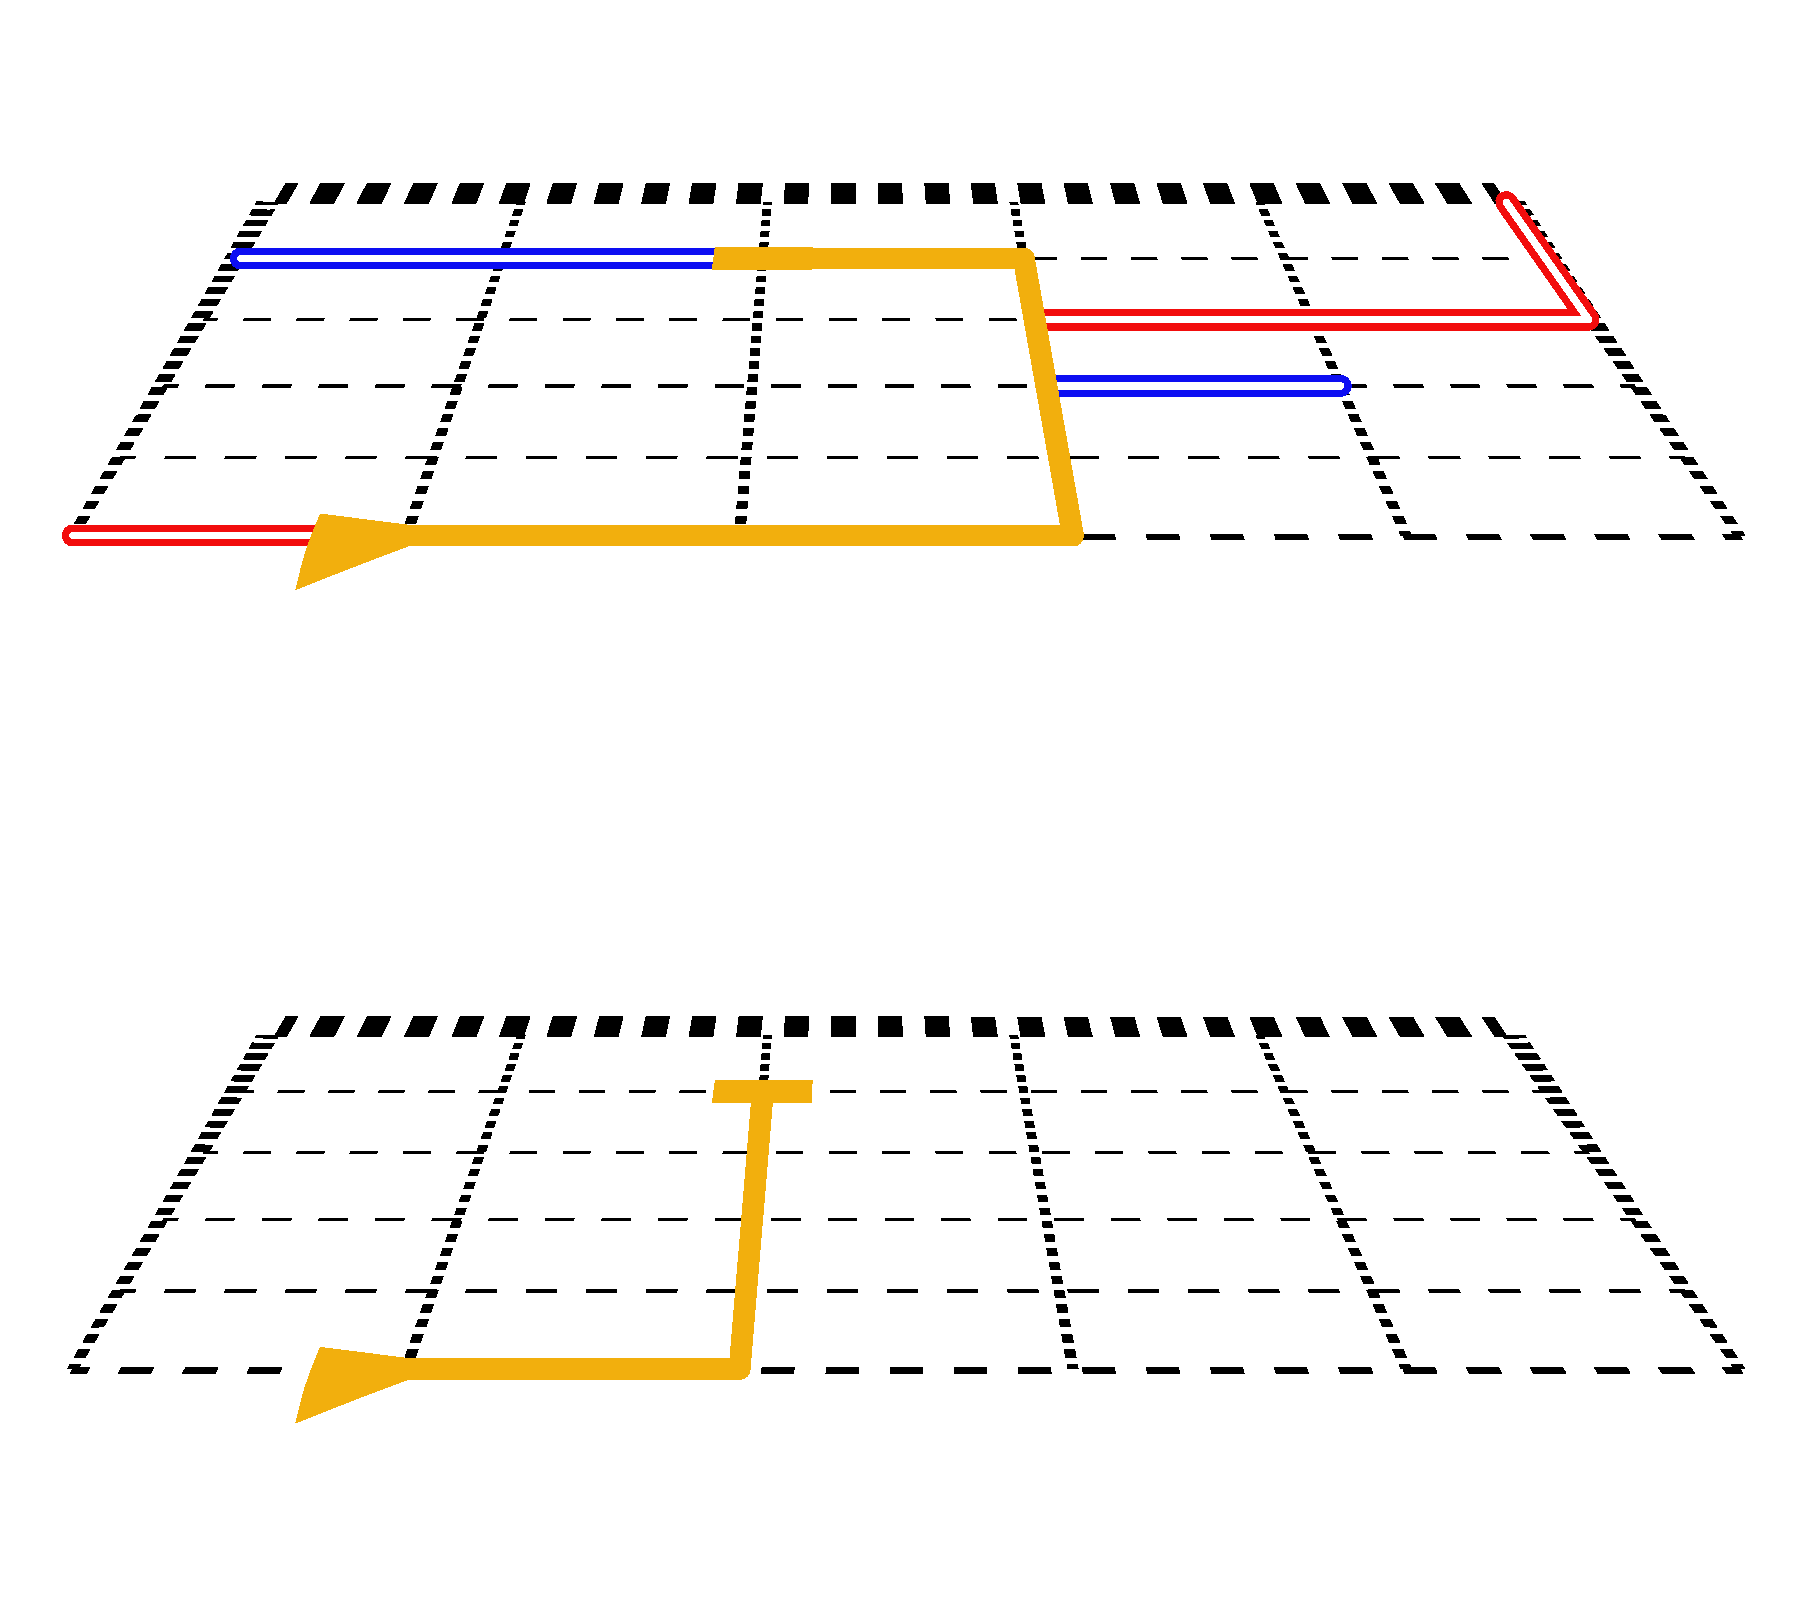
\includegraphics[width=\textwidth]{deux_layers_1.pdf}
			\caption{Shortest paths}
			}
		\end{figure}
	\end{columns}
\end{frame}

\begin{frame}{Modelling trafic (P\&R case)}
	\setbeamercovered{dynamic}
	\begin{columns}
		\column{0.6\textwidth}
		Two layered approach, with connections
		\begin{itemize}
			\item<-2> Park \& Ride facilities serve as connections between the two layers
			\item<2> But, need to enforce only use one P\&R facility \begin{itemize}
				\item[\textrightarrow] Separate onboarding and offboarding links
				\item[\textrightarrow] 3 possible networks
			\end{itemize}
			\item<3> (All-or-nothing assignment) For every group: \begin{itemize}
				\item Compute travel time without light rail
				\item If the origin is at a station, compute travel time with offboarding links 
				\item If the destination is at a station, compute travel time with onboarding links
				\item[$\Rightarrow$] Assign trafic according to the one with the shortest time
			\end{itemize}
		\end{itemize}
		\column{0.4\textwidth}
		\centering
		\begin{figure}
			\centering
			\only<1>{
			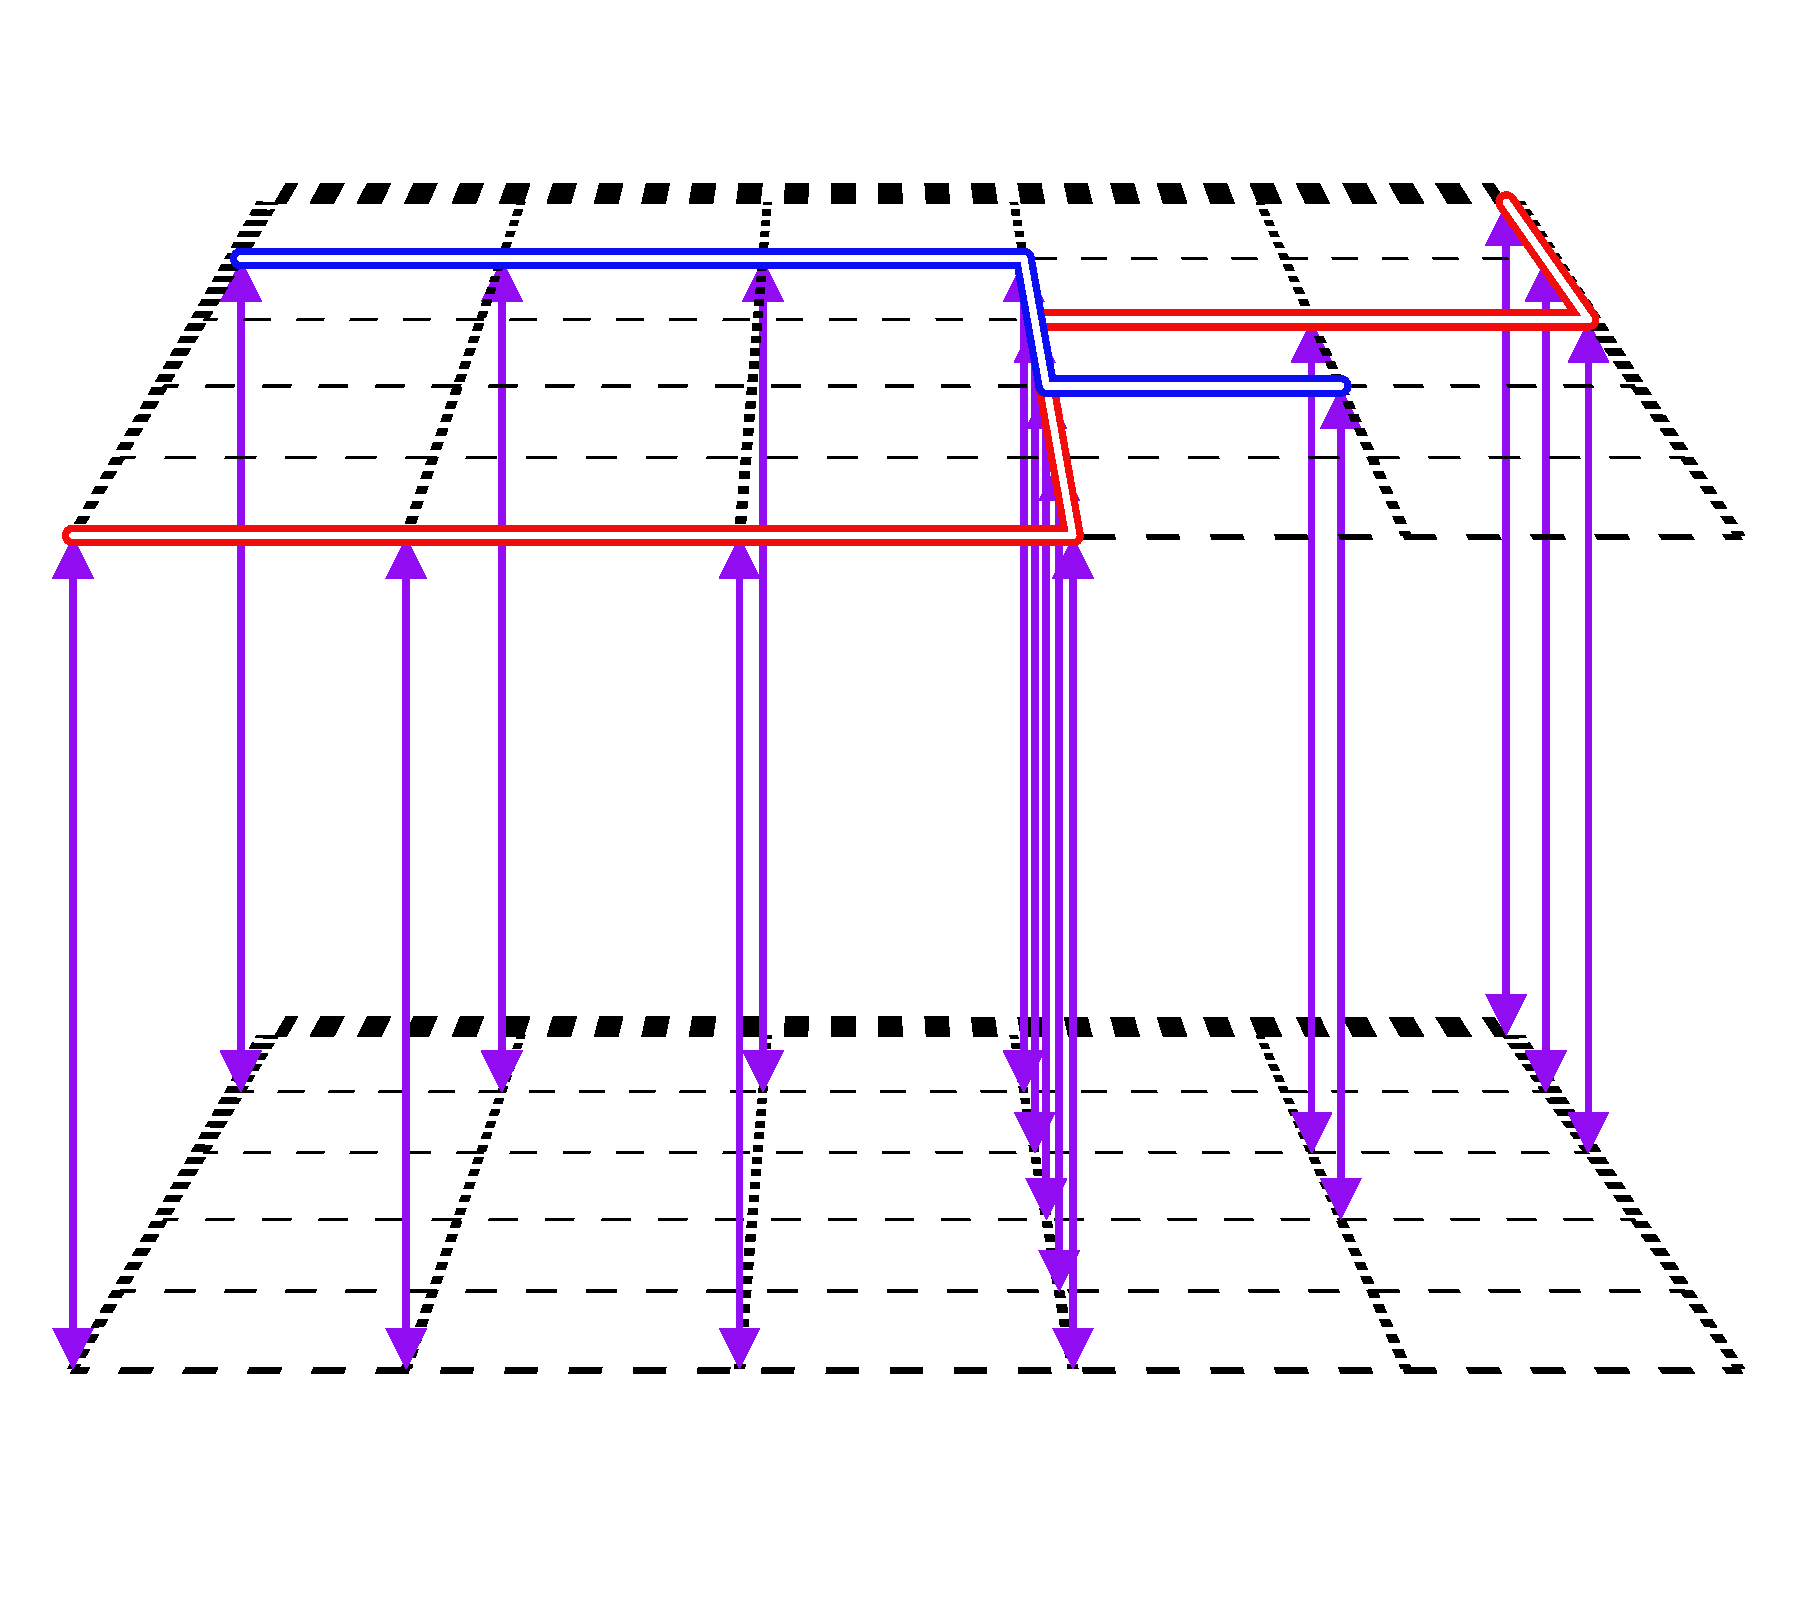
\includegraphics[width=\textwidth]{deux_layers_2.pdf}
			\caption{Two layers approach, with connections}
			} \only<2>{
			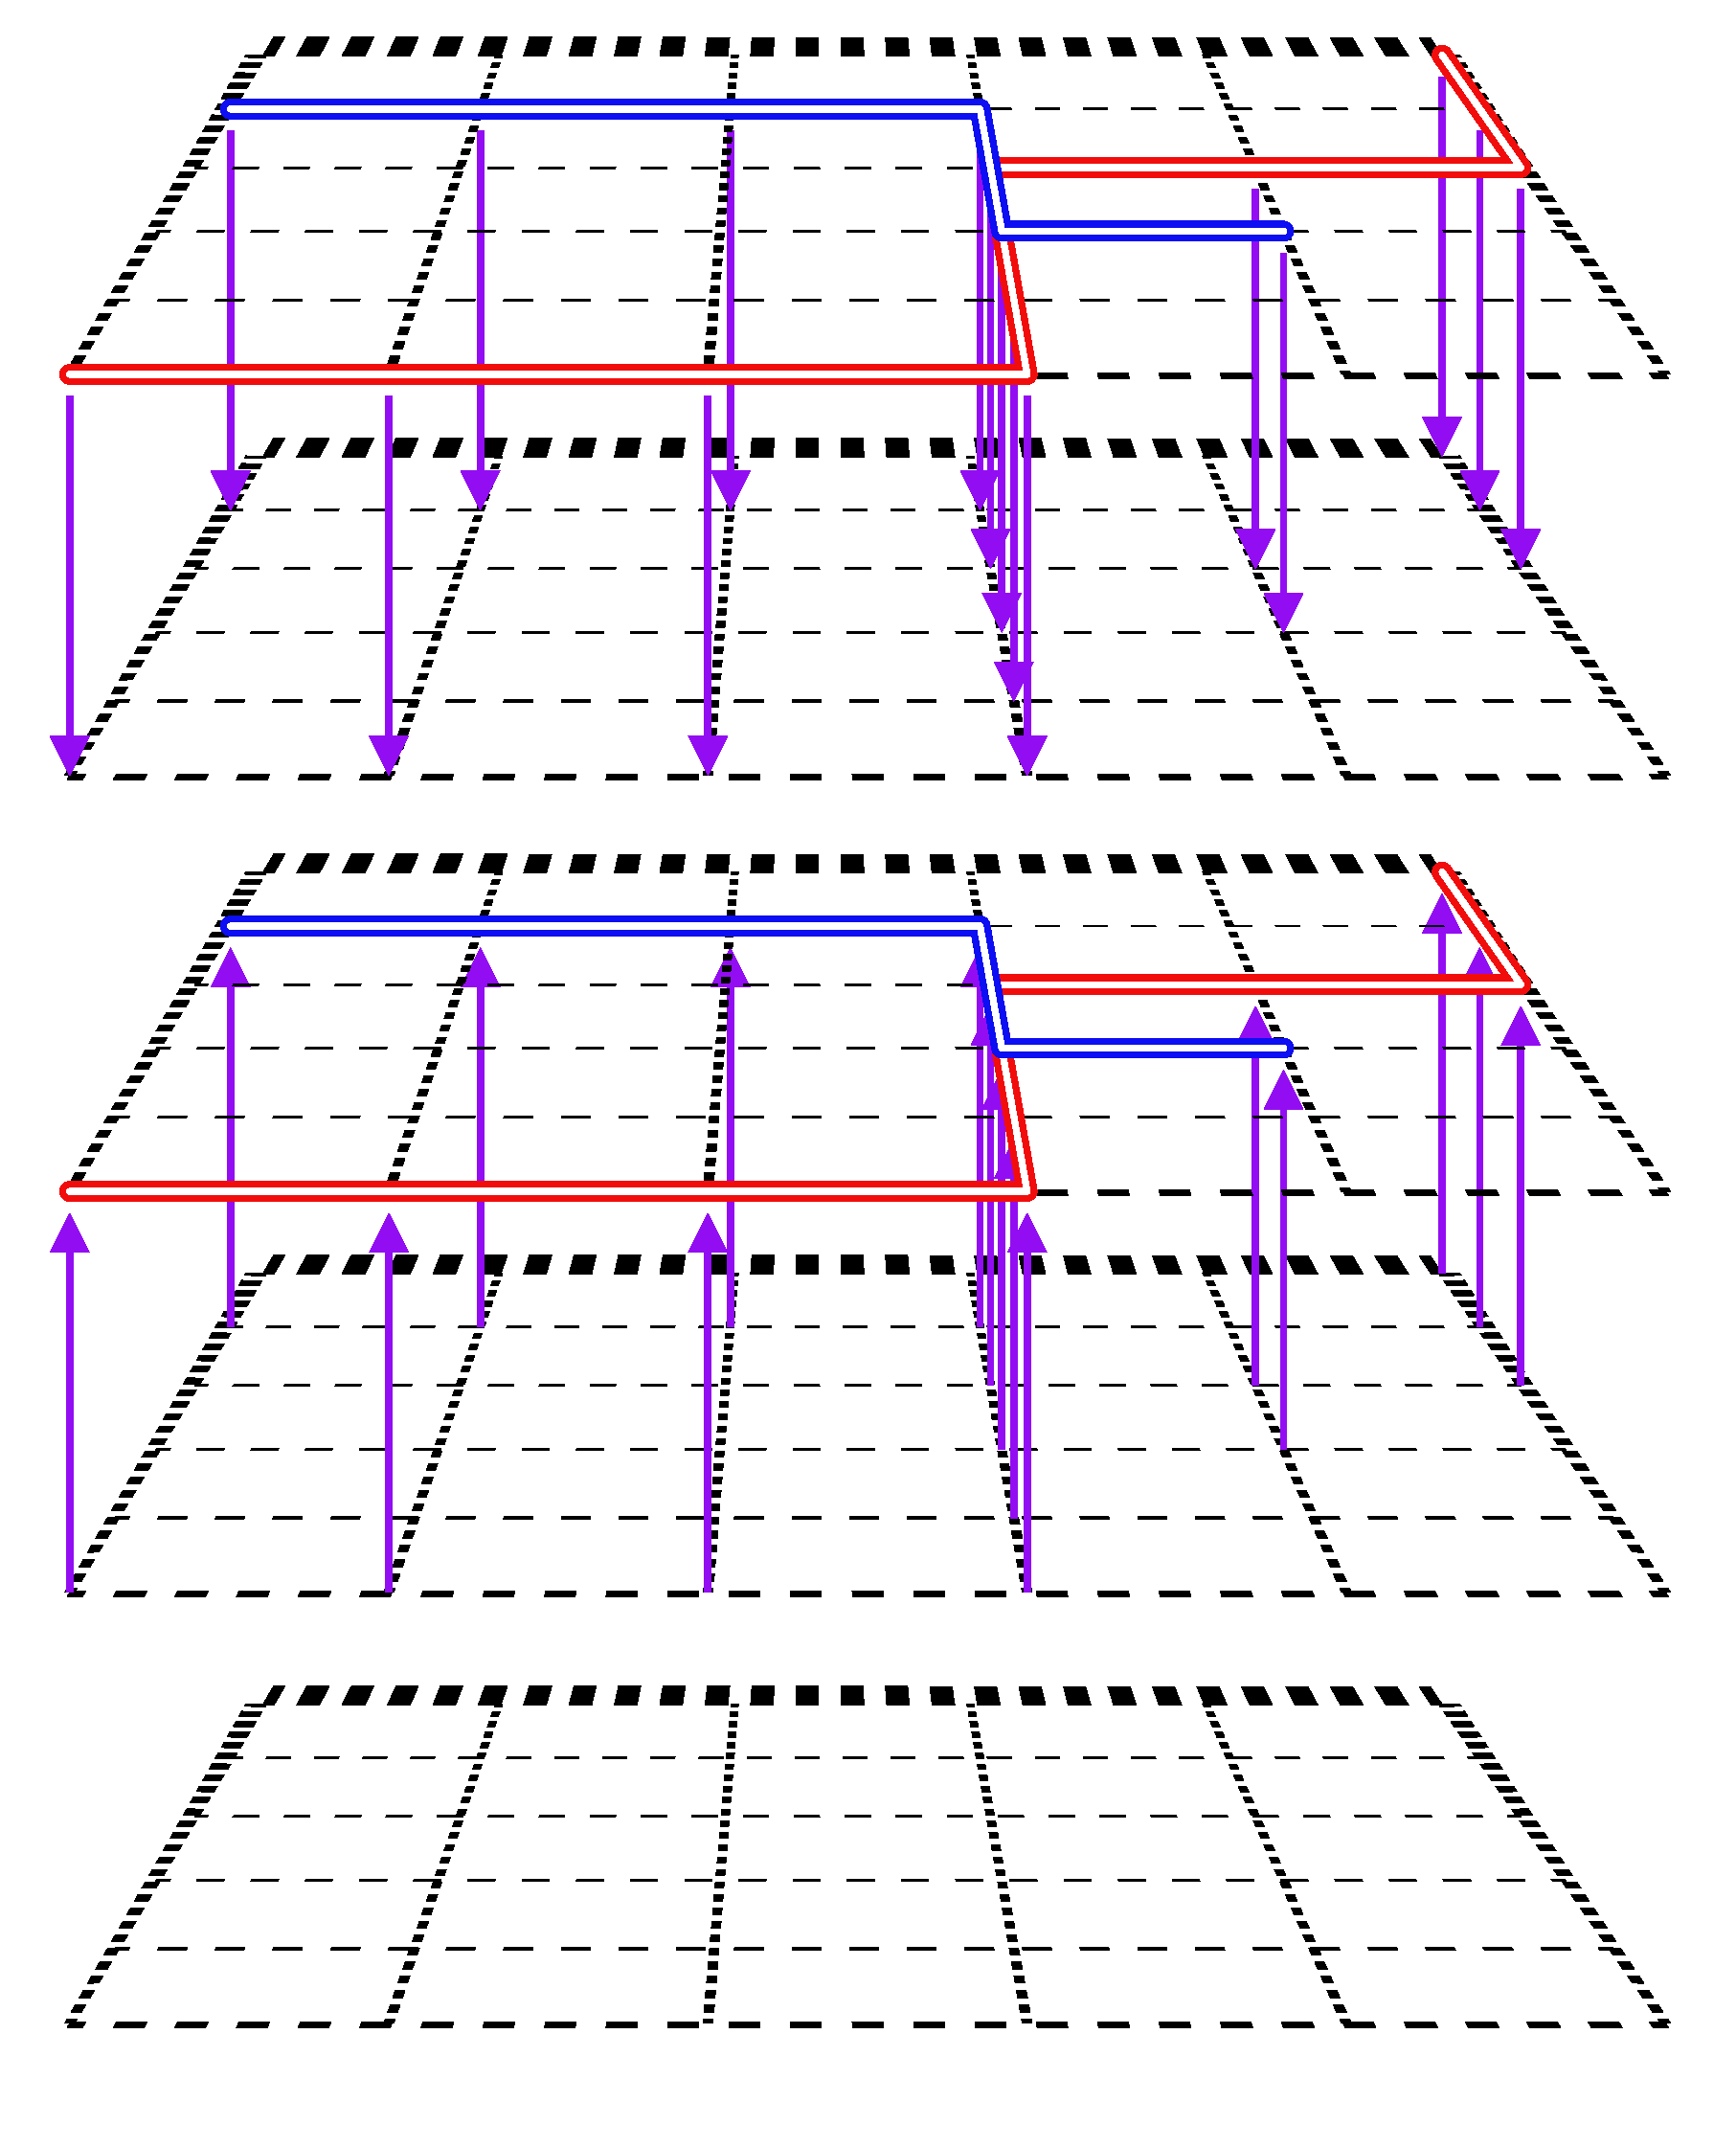
\includegraphics[width=.75\textwidth]{deux_layers_3.pdf}
			\caption{3 networks}
			} \only<3>{
			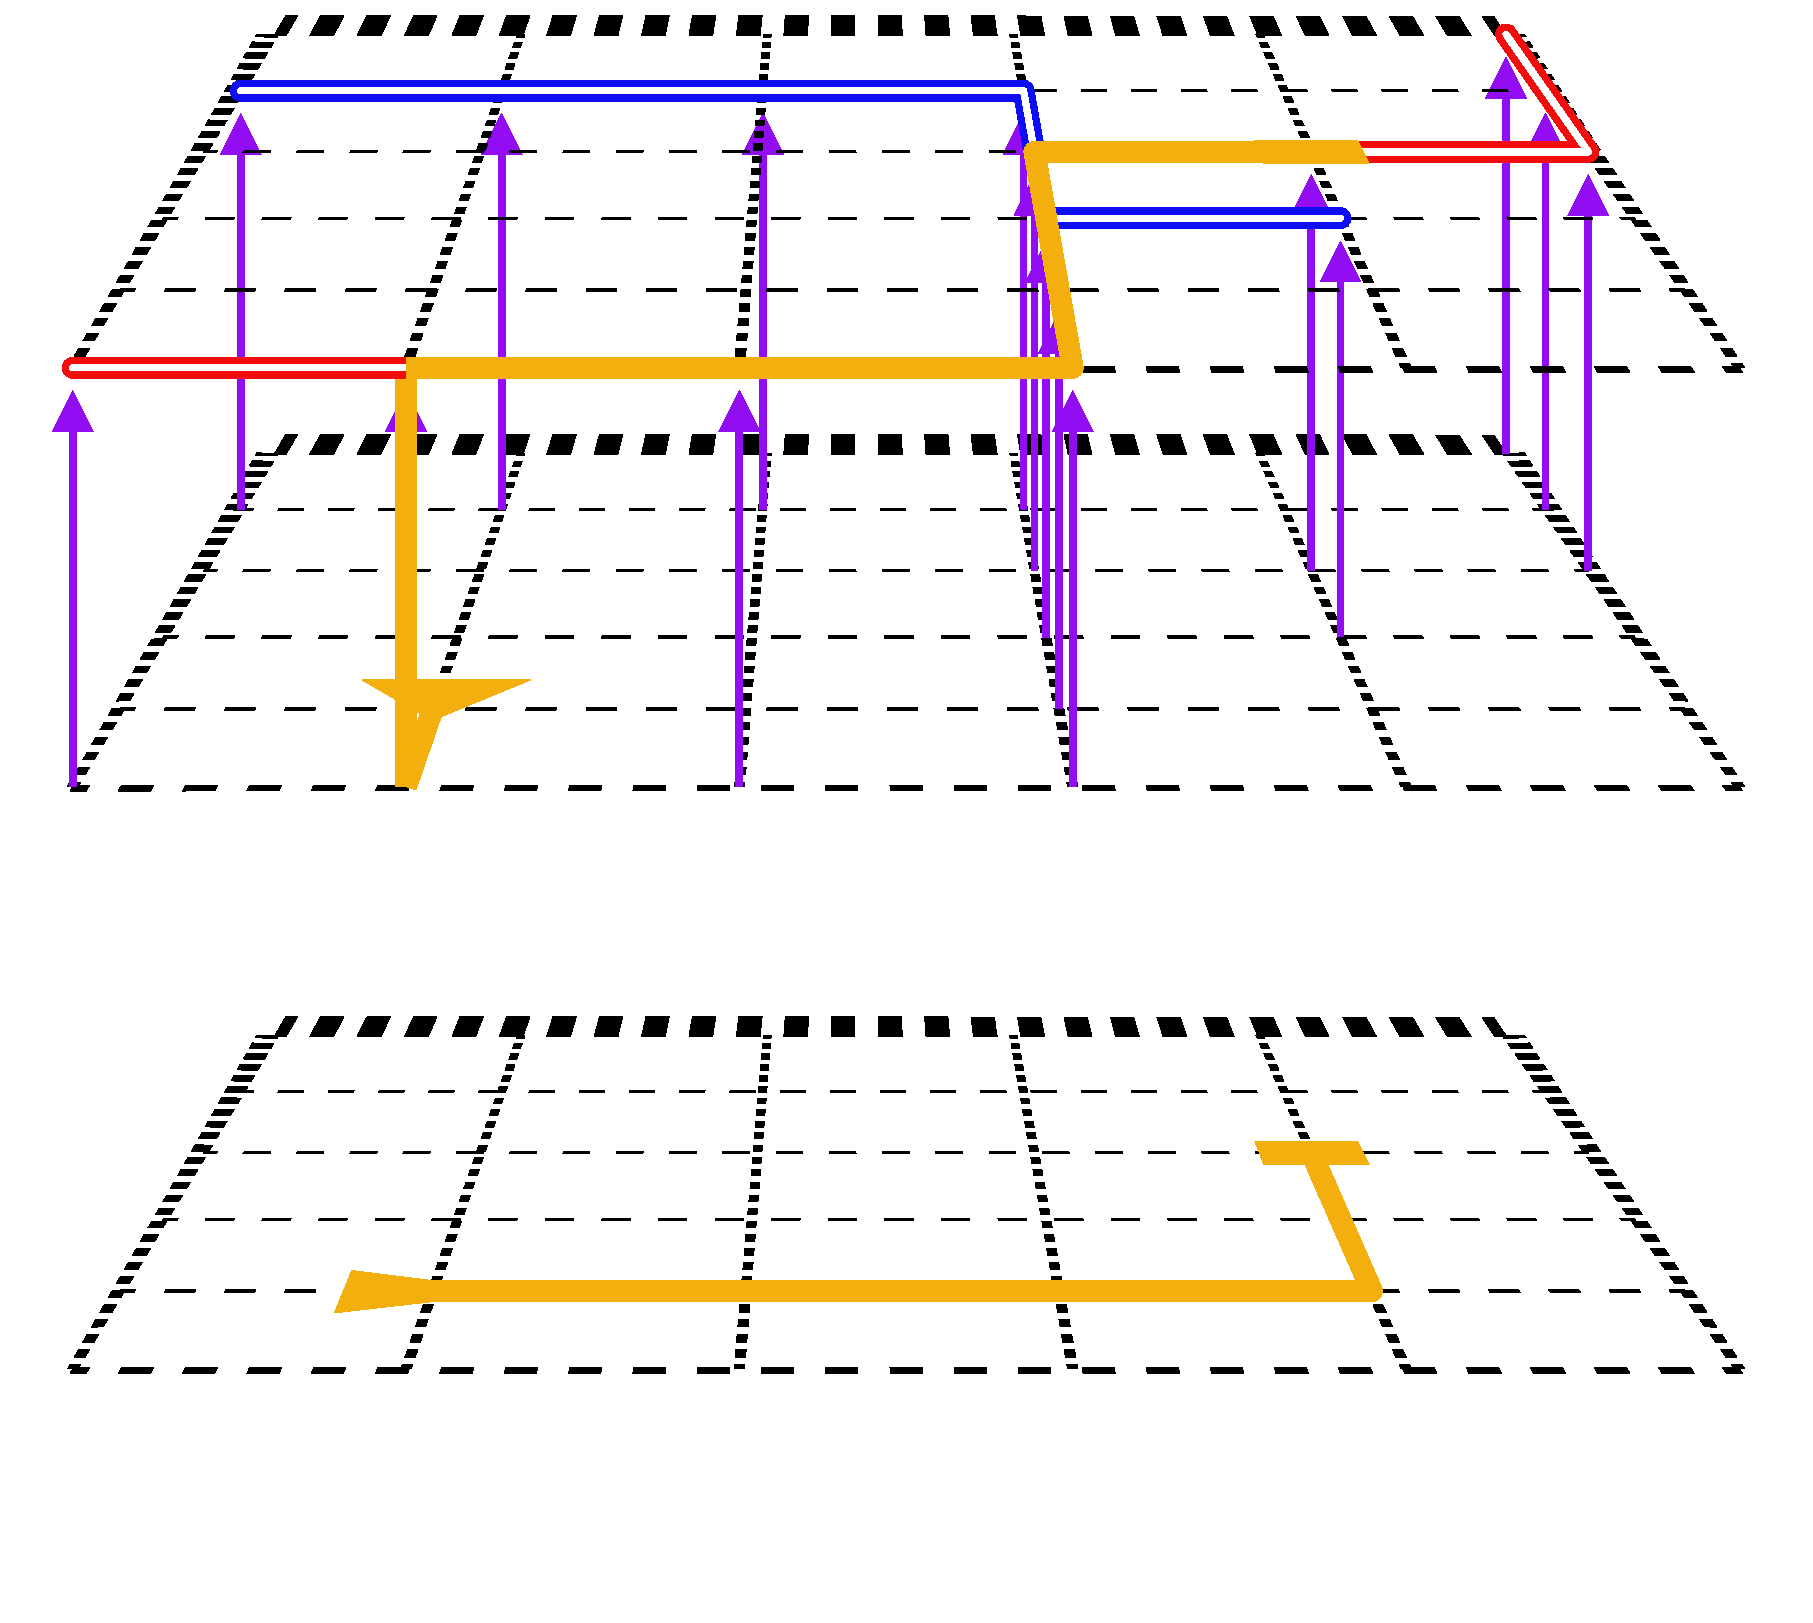
\includegraphics[width=\textwidth]{deux_layers_4.pdf}
			\caption{Shortest path example (onboarding links only)}
			}
		\end{figure}
	\end{columns}
\end{frame}

% --------------------------------------------- Results

\section{Results}
\breakingframe{
\begin{textblock*}{0.8\textwidth}[0,0.5](0.17\textwidth,  0.55\textheight)
\centering \Huge\textbf{\textcolor{black}{Results}}
\end{textblock*}
}

\end{document}